\subsection{Fil beskrivelse}


\subsubsection{XML data dokuments}

\begin{itemize}
\item \textbf{all.xml} Video (�ldre version) Indholder detaljeret information om alle videoer.
\item \textbf{all\_new.xml} Video (nyere version)
\item \textbf{programseries.xml} Programserie (�ldre version) med informationer om alle tilg�ngelige serier.
\item \textbf{programseries\_new.xml} Programserie (nyere version)
\end{itemize}



\subsubsection{XML Skemaer}

\begin{itemize}
\item \textbf{all\_schema.xsd} Skema til all\_x.xml filer
\item \textbf{programseries\_schema.xsd} Skema til programseries\_x.xml filer
\end{itemize}


\subsubsection{XQuery og XPath foresp�rgsler}

\begin{itemize}
\item \textbf{dr\_api\_module.xqm} XQuery modul med de meste af foresp�rgsler
\item \textbf{dr\_api\_module\_usage.xq} Eksempel som viser hvordan modulen dr\_api\_module.xqm bruges.
\item \textbf{word\_cloud\_search.xq} Foresp�rgsel til ord sky funktionen.
\item \textbf{text\_search-Restaurant-laks.xq} Full text s�gning in programserie.
\item \textbf{ful-text-search-SCORE-Restaurant-laks.xq} Full text s�gning in programserie med score information.

\end{itemize}


\subsubsection{Supplerende filer}

\begin{itemize}
\item{stop-words.txt} List med brugte stop ord til full text s�gning.
\end{itemize}



\subsection{BaseX konfiguration}
I projektet blev brugt BaseX 7.8.1.

Opret en ny database i BaseX med \textit{Database - New} kommando for hver fil, programseries.xml, programseries\_new.xml, all.xml og all\_new.xml. Det er vigtigt at i den \textit{Create Database} menu under \textit{Indexes} den Full-Text Index blev aktiveret, sprog dansk og stop-word.txt filen bliver valgt som vist p� figur \ref{inst:BaseXIndex}.

\begin{figure}[h!]
  \centering
   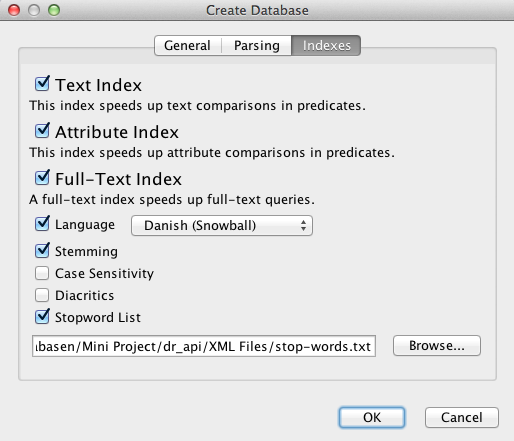
\includegraphics[width=0.8\textwidth]{pic/BaseX-Index.png}
   \caption{BaseX - Full-Text index indstilling }
	\label{inst:BaseXIndex}
\end{figure}

